\documentclass{standalone}

\input{../colours.tex.preamble}
\input{../tikz.tex.preamble}

\begin{document}
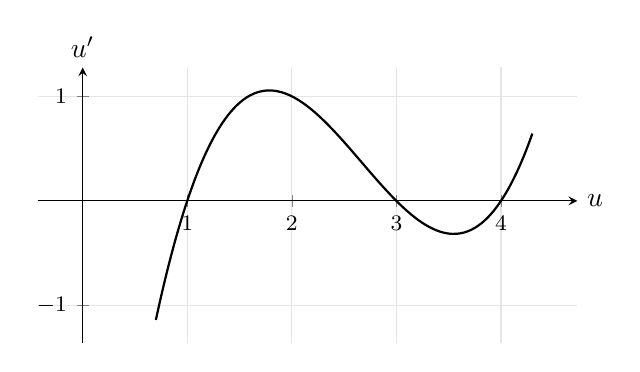
\begin{tikzpicture}
    \begin{axis}[
    axis lines = middle, % boxed, middle
    axis equal image,
    %
    % domain and range
    %
    xmin={0}, % xmax={},
    % ymin={}, ymax={},
    enlargelimits=true,
    %
    % axis labels
    %
    xlabel={\(u\)}, xlabel style={anchor=west},
    ylabel={\(u'\)}, ylabel style={anchor=south},
    label style={at={(ticklabel* cs:1)}},
    %
    % ticks
    %
    % xtick={}, xticklabels={},
    ytick={-1,0,1}, % yticklabels={},
    ticklabel style={font=\footnotesize},
    %
    % grid
    % none, major, minor, both
    grid=major, grid style={gray!20},
    % minor tick num=1, 
    % minor grid style={gray!20},
    % 
    % plot parameters
    %
    smooth, samples=100, no markers,
    ]
    % \usepackage{pgfplots}
    % \pgfplotsset{compat=newest, trig format=rad} 
    % \pgfplotsset{label style={font=\footnotesize}}
    \addplot[thick, domain=0.7:4.3] {(x-1)*(x-3)*(x-4)/2};
    \end{axis}
  \end{tikzpicture}
\end{document}
